\section{Example 2: Data Assimilation}

In the last section we motivated the use of random variables through simple examples involving discrete random variables, in particular six sided dice. These problems were solved internally by constructing and running through iterators as was done in the work by []. In this section we will consider continuous random variables. Instead of iterating through the continuum of possible values we will generate and solve integral expressions. We will see that while the
backend mechanics have been completely changed, the method of setting up a statistical problem remains unchanged. This is a theme upon which we will elaborate in the following sections. 

We consider the problem of data assimilation. On a hot summer day we guess the temperature outside as being about 30C. We're uncertain of this guess so we add on a $\pm3$. We model this with a normal random variable

\begin{lstlisting}
>>> T = Normal(30, 3)
\end{lstlisting}

As in the last section we may ask questions such as $P(T>33)$. These produce integral expressions which are then solved using the SymPy integration engine to produce numeric results.
\begin{eqnarray*}
P(T>33) & = & \int_{33}^{\infty} \frac{\sqrt{2} e^{- \frac{1}{18} \left(x_{3} -30\right)^{2}}}{6 \sqrt{\pi}}\, dx_{3} \\
& = & - \frac{1}{2} \operatorname{erf}{\left (\frac{1}{2} \sqrt{2} \right )} + \frac{1}{2} \\
& = & 0.15866
\end{eqnarray*}

If we are unsatisfied with this single estimate of the temperature we may decide to measure with a thermometer. Our thermometer is difficult to read however (the lines are spaced closely together) and so we understand that our observation will include some noise. 

\begin{lstlisting}
>>> noise = Normal(0, 1.5)
>>> observation = T + noise
\end{lstlisting}

We measure a value of $26C$ and record this as data.

We now have two pieces of information on the same intrinsic value. We have $T$, our \textit{prior} understanding and our new data. We plot them both in Fig. \ref{fig:DA_data}. 

\begin{figure}[ht]
\vspace{-0pt}
\centering
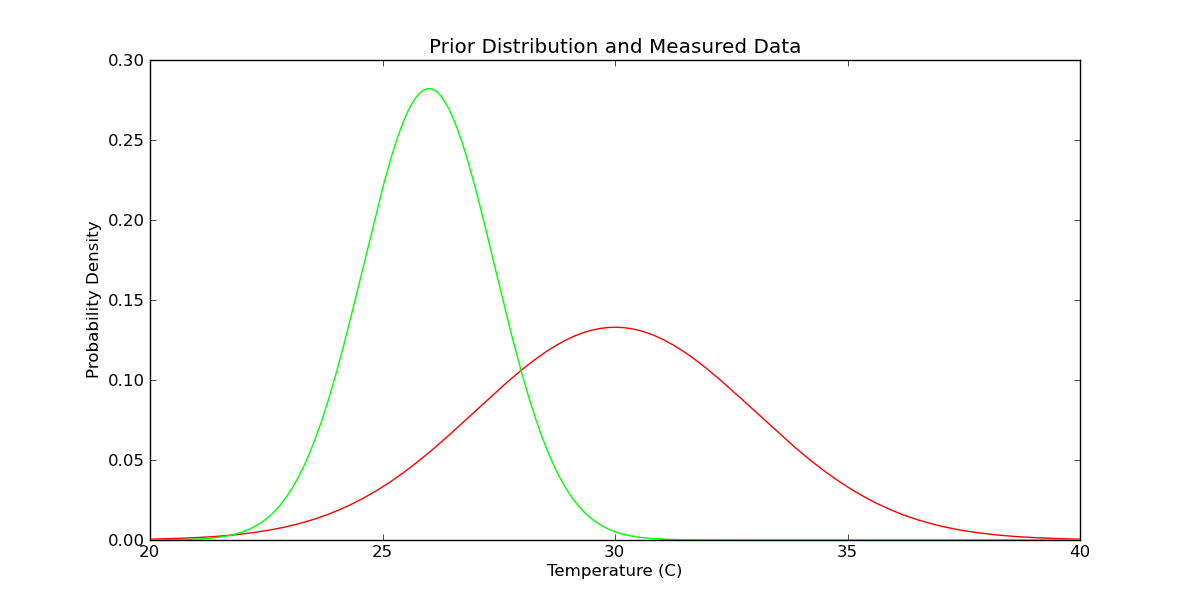
\includegraphics[width=.7\textwidth]{images/data.png}
\vspace{-0pt}
\caption{The probability density functions of our two pieces of data. Note that the observation is less uncertain and thus more centered about the mean.}
\label{fig:DA_data}
\vspace{00pt}
\end{figure}

After we make this measurement how should our final estimate of the temperature change? We have the original estimate, $30C \pm 3C$, and the new measurement $26C \pm 1.5C$. We could take the thermometer’s reading because it is more precise but this doesn’t use the original information at all. The old measurement still has useful information and it would be best to cleanly assimilate the new bit of data $(26C \pm 1.5C)$ into our prior understanding $(30C \pm 3C)$

This is the problem of Data Assimilation. We want to assimilate a new measurement (data) into our previous understanding (prior) to form a new and better-informed understanding (posterior). Really, we want to compute $T' = T$ given observation $= 26$. We compute this in SymPy as follows

\begin{lstlisting}
>>> T_posterior = Given(T, Eq(observation, 26))
\end{lstlisting}

The new distribution is plotted in Fig. \ref{fig:DA_posterior}. The exact functional form is proportional to $e^{-\frac{2}{9} \left(-x + 26\right)^{2}} e^{-\frac{1}{18} \left(x-30\right)^{2}}$ 

\begin{figure}[ht]
\vspace{-0pt}
\centering
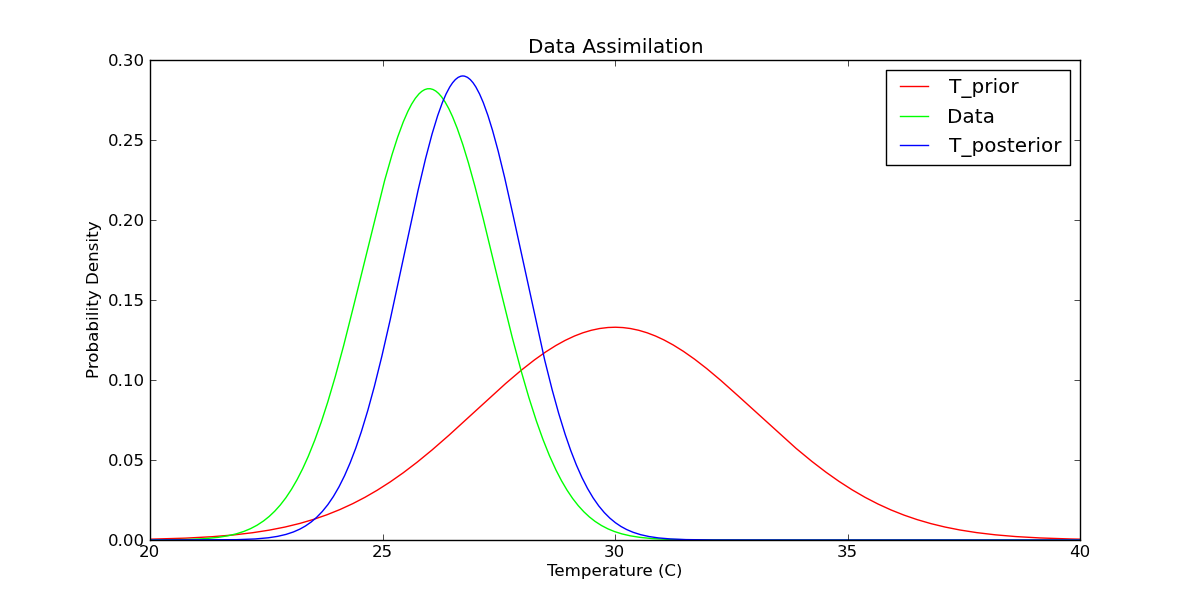
\includegraphics[width=.7\textwidth]{images/posterior.png}
\vspace{-0pt}
\caption{The density of the posterior represents our understanding after the observation has been assimilated into our prior understanding. Note that it is more centered/certain than either of the two. }
\label{fig:DA_posterior}
\vspace{00pt}
\end{figure}

This is a classic result in data assimilation. It is important to note that these rules are not directly written into SymPy. Rather this is \textit{the} answer given the most basic and fundamental rules. 
